\chapter{System Model}
\label{ch:sysmodel}

As mentioned in Chapter \ref{ch:intro}, the goal of this thesis is to collect the measurement data from the MIMO setup. This collected experimental data will be applied to the machine learning model which has been developed in parallel with this thesis. In this chapter the relevant fundamentals of the LTE standard, which will be used as a basis for our channel estimation are described on a high level.

%\par
%
%In the following sections we would discuss the LTE frame structure and the relevant signalsthat are required for the collection of the data. The release of the LTE standard being used here is the Release 10.

\section{LTE}\label{sec:LTEProc}

LTE stands of Long Term Evolution and is a successor standard to UMTS. LTE is a multicarrier approach for multiple access which uses Orthogonal Frequency-Division Multiple Access (OFDMA) in the physical layer. OFDM uses multiple carriers (known as sub carriers) spaced equally apart and can transmit independent data streams on each sub carrier \cite{rohling}.

\par

Hence an LTE frame is commonly represented as a 2D time frequency grid, where the vertical axis represents the sub-carriers(Frequency) and the horizontal axis represents time. LTE also comes in 2 flavours Frequency Division Duplexing (FDD) and Time Division Duplexing (TDD). In this thesis the focus will be on FDD systems, which use seperate frequency bands, for uplink and for downlink data respectively. The advantage of an FDD system is that the uplink and downlink transmittion can happen simultaneously.

LTE has a certain predefined signal symbol structure according to the standard \cite{3gpp36211}. In the following sections the frame structure and the different symbols in the LTE Frame shall be introduced.

\section{LTE Waveform Processing}\label{sec:LTE Waveform Processing}
LTE stands of Long Term Evolution and is a successor standard to UMTS. LTE is a multicarrier approach for multiple access which uses Orthogonal Frequency-Division Multiple Access (OFDMA) in the physical layer. OFDM uses multiple carriers (known as sub carriers) spaced equally apart in frequency and can transmit independent data streams on each sub carrier \cite{rohling}. LTE also comes in 2 flavours Frequency Division Duplexing (FDD) and Time Division Duplexing (TDD). In this report the focus will be on FDD systems, which uses seperate frequency bands for uplink and for downlink data so that the uplink and downlink data can be transmitted simultaneously.

LTE was chosen as a standard to use for the communication system given the integrated support of simulation environments like MATLAB and Simulink and that it is currently widespread in the telecommunications industry.

\subsection{Transmission} \label{ssec:Transmission}

A dual antenna transmitter using a USRP software defined radio as mentioned in \ref{sec:USRP} is used for the interface. A modified version of the LTE Application framework with MIMO 2x2 extension is used to log the data and run with different parameters. The transmitter USRP is connected to a Host PC using a 4-lane PCIe connection. This is necessary for the high data throughput exchanged between the host and the devices.

LTE has a standardized frame structure which is commonly represented as a 2D time frequency grid, where the vertical axis represents the sub-carriers and the horizontal axis represents time. LTE also uses a predefined signalling structure according to the standard \cite{3gpp36211}. In the following sections the frame structure and the symbols relavent to channel estimation shall be introduced.

\subsubsection{LTE Frame} \label{LTEFrame}

A single frame is 10ms long and consists of 10 smaller units called subframe, each 1ms long. A symbol is the smallest unit of time for an LTE system and one subframe has 14 such symbols each approximately 66.7us long. Scheduling is normally done on a subframe basis for both uplink and downlink communication.

LTE's time frequency grid contains many different signals each performing specific funtionality like broadcasting, control channel information, data transfer, among other functions.

For the puprpose of channel estmation, the most important signals are Primary Synchronisation Signal(PSS), Secondary Synchronisation Signal (SSS) and Cell Specific Reference Signal (CRS) which are described in detail in the subsequent sections.

\subsubsection {Primary Synchronisation Signal (PSS)} \label{sssec:PSS}
        OFDM is extremely time and frequency sensitive, hence it is very important to know the exact start of every frame. The PSS helps to achieve the synchronisation of the frame by using a specific sequence called the Zadoff-Chu sequence \cite{3gpp36211}.
        The Zadoff-Chu sequence has the property of constant amplitude zero autocorrelation waveform (CAZAC sequences) that cyclically shifted versions of the waveform are orthogonal to each other. The sequence is described in Equation \ref{eq:ZCSeq} where {\em u}  can be 25,29 or 34 depending on the cell ID.
        The PSS is broadcast twice every radio frame and the symbols are identical each time.

\begin{equation} \label{eq:ZCSeq}
        d_u(n) =
        \begin{cases}
            \mathrm{e}^{-j\frac{\pi un(n+1)}{63}}       & \quad n=0,1,...,30\\
            \mathrm{e}^{-j\frac{\pi un(n+1)(n+2)}{63}} & \quad n=31,32,...,61
        \end{cases}
\end{equation}

\subsubsection{Secondary Synchronisation Signal (SSS)} \label{sssec:SSS}
        The SSS is a 62 bit pseudo random sequence \cite{3gpp36211}. It is broadcast twice in a frame once in subframe 0 and once in subframe 5, one symbol before the PSS. The 2 sequences of transmission in a frame are different so that the UE can identify which position in the frame the synchronisation happens.

\subsubsection{Cell Specific Reference Signal (CRS)} \label{sssec:CRS}
        As mentioned in Chapter \ref{ch:intro} the channel needs to be estimated in order to reverse the channel propogation effects. With the help of CRS the channel can be estimated by placing equally spaced reference symbols along every 6 subcarriers starting from subcarrier 2 on symbols 1, 8, 15, etc... and every 6 subcarriers starting from subcarrier 5 on symbols 5, 12, 19, etc...\cite{3gpp36211}. The signals received by the UE and the channel effects are inferred based on amplitude damping and phase shift. Placing the signals in the above defined spacing gives the best coverage to interpolate over in time and frequency.

        The signals to be placed on the grid are decided by the Equation \ref{eq:CRS} as shown below, with the parameters defined in Table \ref{tab:CRSParam} \cite{3gpp36211}.
        \begin{equation} \label{eq:CRS}
            r_{l,n_s}(m) = \frac{1}{\sqrt{2}}(1-2{\cdot}c(2m)) + j\frac{1}{\sqrt{2}}(1-2{\cdot}c(2m+1)),\ m=0,1,...,2N_{RB}^{max,DL}-1
        \end{equation}

        \begin{table}[H]
            \begin{center}
                \begin{tabular}{|l|l|}
                    \hline
                    Parameter& Description\\ \hline
                    $c(m)$& Pseudo Random Sequence defined in \cite{3gpp36211}\\ \hline
                    $N_{RB}^{max,DL}$& Maximum number of Downlink resources blocks\\ \hline
                    $n_s$& Slot number in the frame\\ \hline
                    $l$& OFDM Symbol number in the frame\\
                    \hline
                \end{tabular}
                \caption{Parameter definitions for evaluating CRS Symbols}
                \label{tab:CRSParam}
            \end{center}
        \end{table}

\subsubsection{PDCCH}

%//TODO add the time domain and spectrum figure

\subsubsection{Final Waveform}
All the signals mentioned in Section \ref{LTEFrame} are generated in Labview using the LTE Application Framework Software and arranged in a 2D grid of frequency and time as shown below in Figure \ref{fig:RBSignals}. The CRS are placed every 6 subcarriers in the frequency domain and every 3 or 4 time symbols apart, according to the position on the grid. Where as the PSS and SSS only repeat every 5 subframes.

\begin{figure}[H]
    \begin{center}
        %\includegraphics[wisdth=\linewidth]{../ReportImages/RB_legend.jpg}
        \caption{Resource Block Grid for 2 sub frames}
        \label{fig:RBSignals}
    \end{center}
\end{figure}

One of the disadvantages of using OFDM in the physical layer is the high peak to average power ratio (PAPR) of the signal. High PAPR translates to high fidelity requirements of power amplifiers on the transmitter side. It also induces non-linear distortions to the signal \cite{rohling}. To ensure that the PAPR of the signal is as low as it can be, random QPSK symbols are transmitted on the unused slots instead of 0s.

\subsection{Reception}

For the LTE receiver processing a USRP captures in bursts and streams the data to a laptop connected via a USB interface. The signals are processed by a custom MATLAB application which performs the necessary steps to decode the LTE Frames, estimate the channel and display the information as a 3D surface. For the case of the demo the data was processed as soon as they were received from the USRP and the channel estimate was displayed in realtime. The data can alternatively be logged for offline postprocessing to get better granularity as intermittent processing delays dont appear.

Once enough samples have been captured (usually 2 or more Frames) the data can be processed in the following steps.


\subsubsection{Carrier Offset Estimation and Correction}
OFDM is extremely senstive to frequency shifts in the received signal. In the case that the receiver or transmitter center frequency clock was not accurate enough, the frequency shift needs to be estimated and corrected. This is the very first step before processing the baseband waveform.

%TODO

\subsubsection{Frame synchronisation}
As mentioned in Section \ref{LTEFrame} the synchronisation is a very important part of knowing where the LTE frame begins. This is done by correlating the received signal with the known Zadoff Chu Sequence and to look for the peak. Figure \ref{fig:PSSCorr} shows an example correlation of a Zadoff Chu sequence and a received signal containing 307200 samples in total amounting to 2 frames of a 10MHz Bandwidth LTE signal. 4 peaks are to be expected here as there are 2 frames, each containing 2 PSS sequences.

\begin{figure}[H]
    \begin{center}
        %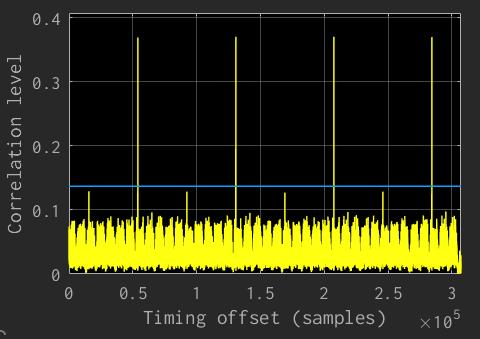
\includegraphics[width=9cm]{../ReportImages/PSSCorrelation.jpg}
        \caption{PSS Correlation}
        \label{fig:PSSCorr}
    \end{center}
\end{figure}

\subsubsection{Channel Estimation}

Once the frame has been demodulated and the 2D OFDM grid has been obtained, the channel can be estimated based on the original pilot symbols structure known to the receiver, hence the phase and amplitude of the particular sub carrier can be obtained. A 2D wiener filter is applied in both the time and frequency axis to interpolate the channel estimate. More explained in the Chapter \ref{ch:ChEst}.

%TODO

\subsection{Antenna}
The analog time domain signal is transmitted from the USRP (Section \ref{sec:USRP}) over the air using a Triband antenna. For the setup an omni directional Antenna from TODO capable of transmitting and receiving around frequencies of 144, 400 or 1200 MHz. This antenna shown in Figure \ref{fig:USRPAnt} was used as the transmit and the receive antenna for the demo setup.

\begin{figure}[H]
    \begin{center}
        %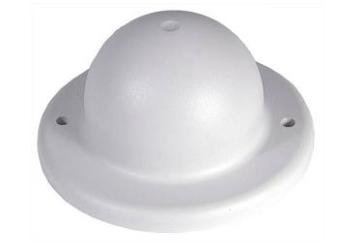
\includegraphics[width=7cm]{../ReportImages/HuberAntenna.png}
        \caption{Wideband Omnidirectional Antenna used for transmitting and receiving the LTE Signals}
        \label{fig:USRPAnt}
    \end{center}
\end{figure}
